\documentclass[conference]{IEEEtran}
\IEEEoverridecommandlockouts
\usepackage{cite}
\usepackage{amsmath,amssymb,amsfonts,amsthm}
\usepackage{algorithmic}
\usepackage{algorithm}
\usepackage{graphicx}
\usepackage{textcomp}
\usepackage{xcolor}
\usepackage{booktabs}
\usepackage{array}
\usepackage{multirow}
\usepackage{url}

\newtheorem{theorem}{Theorem}
\newtheorem{proposition}{Proposition}
\newcommand{\cerca}{CERCA}
\newcommand{\ms}{\,ms}
\newcolumntype{C}[1]{>{\centering\arraybackslash}p{#1}}
\newcolumntype{L}[1]{>{\raggedright\arraybackslash}p{#1}}

\begin{document}

\title{CERCA: Context-Aware Root Cause Analysis Under Degraded Telemetry in Microservice Architectures}

\author{
\IEEEauthorblockN{Harshil Khanna}
\IEEEauthorblockA{\textit{School of Computer Science and Engineering}\\
\textit{Vellore Institute of Technology}\\
Vellore, India\\
harshil.khanna2023@vitstudent.ac.in}
\and
\IEEEauthorblockN{Charvi Sood}
\IEEEauthorblockA{\textit{School of Computer Science and Engineering}\\
\textit{Vellore Institute of Technology}\\
Vellore, India\\
charvi.sood2023@vitstudent.ac.in}
}

\maketitle

\begin{abstract}
Automated root cause analysis (RCA) in distributed microservice architectures is a critical operational challenge. Existing methods, including time-series correlation, iterative graph random walks, and causal-model approaches, assume dense and complete observability. Yet real-world cloud deployments routinely suffer from dropped distributed traces, delayed metric scrapes, and partially unavailable monitoring infrastructure when failing containers crash. This paper presents CERCA (Context-Aware Empirical Root Cause Analysis), an efficient two-tier inference framework that combines direct telemetry evidence with upstream contextual surrogate blame propagated backward across the service dependency graph. We formalize context-awareness across six operational dimensions, state a Positive Upstream Blame Propagation Guarantee showing that a completely silent root-cause service receives strictly non-zero diagnostic blame from caller distress signals, and prove exact Rank-1 identifiability conditions with fan-in normalisation to mitigate hub-centrality masking. Evaluated on the DeathStarBench Social Network benchmark under a progressive 0\%--90\% telemetry degradation ladder, CERCA maintains robust fault localization (MRR 0.3451 at 20\% data loss and 0.2946 at 90\% loss), whereas the MicroRCA baseline collapses to 0.0\% Top-1 recall at just 10\% loss. An incident-level paired Wilcoxon signed-rank test ($N=7$) confirms a statistically significant robustness advantage at 20\% degradation ($W=20.0$, $p=0.0313$; 95\% bootstrap CI $[+0.025, +0.344]$). CERCA also achieves a $39.9\times$ end-to-end execution speedup (26.13\,ms versus 1041.96\,ms per incident) through an $O(|V|+|E|)$ single-pass reverse traversal that avoids the PageRank sink-trap bias.
\end{abstract}

\begin{IEEEkeywords}
root cause analysis, microservices, telemetry degradation, observability, distributed tracing, fault localization, graph propagation
\end{IEEEkeywords}

%% ============================================================
\section{Introduction}
%% ============================================================

Modern cloud-native applications are composed of dozens to thousands of independently deployable microservices communicating over REST, gRPC, and Thrift RPCs. When an incident occurs, such as a CPU-starved service, a memory-exhausted container, or an abrupt process crash, automated root cause analysis (RCA) must rapidly pinpoint the responsible container to meet strict mean-time-to-recovery (MTTR) service-level objectives \cite{chen2014}. The fundamental operational obstacle is that real production environments are frequently \textit{observability-impaired}: Prometheus scrapers miss target pods, Jaeger samplers drop large proportions of spans under burst load, and crashing services often take their monitoring sidecars down with them. Failure diagnosis for such distributed systems has been surveyed extensively \cite{zhang2024survey}, highlighting the growing importance of graph-based models \cite{nguyen2022} and dedicated failure detection mechanisms \cite{tariq2026}.

Existing state-of-the-art RCA frameworks, such as MicroRCA \cite{wu2020}, CloudRanger \cite{wang2018}, Microscope \cite{lin2018}, and $\epsilon$-Diagnosis \cite{shan2019}, are engineered under the fragile assumption of complete, pristine observability. They rely on continuous cross-correlation across synchronized metric series and multi-step random walks across service dependency graphs. As our empirical evaluations demonstrate, these methods suffer a catastrophic collapse under data loss: even a 10\% telemetry blackout severely distorts correlation vectors and prevents personalized PageRank (PPR) random walks from converging to true fault locations, dropping Top-1 recall to 0\%. While recent research models failure propagation via dynamic causality and learned hypergraphs \cite{xie2023impact,zhang2025dyna,xie2025hyper}, these techniques continue to demand high-fidelity, complete inputs and do not formally address partial observability.

CERCA targets this gap directly. The primary contributions of this work are as follows:
\begin{enumerate}
    \item \textbf{Formalization of Contextual Dimensions}: We formulate six operational dimensions of context (topology, upstream behavior, telemetry reliability, operational baselines, temporal windows, and edge coupling) that govern root-cause ranking under degraded observability.
    \item \textbf{Theoretical Foundation}: We state and prove the \textit{Positive Upstream Blame Propagation Guarantee}, establishing that even when a root-cause service is completely silent ($L_{\mathrm{direct}}(s^*)=0$), upstream caller symptoms guarantee a strictly positive blame score. We further derive Proposition~\ref{prop:identifiability} specifying exact Rank-1 identifiability criteria and establish fan-in normalisation to eliminate hub-centrality masking.
    \item \textbf{Sink-Trap-Free Linear Inference}: We design an $O(|V|+|E|)$ single-pass reverse propagation algorithm that completely avoids the sink-trap bias inherent to iterative PageRank, delivering a $39.9\times$ end-to-end execution speedup over MicroRCA.
    \item \textbf{Controlled Degradation Benchmarking}: We evaluate CERCA across a 10-tier controlled degradation ladder (0\%--90\% data loss) on the DeathStarBench Social Network testbed across labeled fault incidents.
    \item \textbf{Methodologically Rigorous Statistical Analysis}: We conduct incident-level paired Wilcoxon signed-rank tests ($N=7$) with 5{,}000-sample bootstrap confidence intervals, demonstrating statistically significant robustness under 20\% telemetry loss ($p=0.0313$).
\end{enumerate}

%% ============================================================
\section{Literature Survey}
%% ============================================================

Root cause analysis in distributed microservices has progressed through several distinct paradigms, thoroughly surveyed in \cite{zhang2024survey} and \cite{nguyen2022}.

\subsection{Metric-Based and Statistical Approaches}
$\epsilon$-Diagnosis \cite{shan2019} clusters request-level performance metrics in short time windows to diagnose microservice latency anomalies. Microscope \cite{lin2018} applies causal inference to trace latency spikes across service call chains. Dapper \cite{sigelman2010} established the distributed tracing foundations on which downstream performance analysis depends. However, these methods depend on continuous telemetry; dropped metrics or truncated traces corrupt the underlying statistical distributions.

\subsection{Graph-Based and Random-Walk Approaches}
CloudRanger \cite{wang2018} constructs correlation graphs from time-series metrics and applies second-order random walks. MicroRCA \cite{wu2020} integrates container metrics with trace graphs, deploying personalized PageRank (PPR) seeded by anomaly detection. However, PPR is an iterative diffusion process: when an anomalous root-cause service is a terminal leaf or suffers telemetry blackout, probability mass diffuses toward arbitrary network sinks, causing innocent nodes to be blamed. Sage \cite{bhagwan2020} leverages predictive ML models over graphs, but requires massive historical data unsuitable for zero-day faults.

\subsection{Log-Based and Anomaly Detection Approaches}
LogCluster \cite{vaarandi2015} and Drain \cite{he2017} parse unstructured log streams into structured templates for anomaly detection. Soldani et al.\ \cite{soldani2024} analyze microservice cascading failures from logs. Nevertheless, log-based diagnosis fails entirely when a crashed container ceases log emission, motivating CERCA's caller-side surrogate blame strategy.

\subsection{Multimodal and Graph-Learning Approaches}
MicroRank \cite{yu2021} merges metrics, traces, and logs using spectrum analysis. Deep learning has also been explored for architectural risk and anomaly detection \cite{abdulsatar2025,wu2026dl}. Recent advances utilize graph neural networks and structural learning: ImpactTracer \cite{xie2023impact} tracks fault propagation, DynaCausal \cite{zhang2025dyna} constructs dynamic causal graphs, and Xie et al.\ \cite{xie2025hyper} formulate hypergraph conditional learning. MTG-CD \cite{chen2024mtgcd}, Xue et al.\ \cite{xue2026}, Li \cite{li2026}, ServiceGraph-FM \cite{zeng2026}, and ST-GraphRCA \cite{su2026} introduce rich structural representations. While effective under ideal conditions, these models require dense feature tensors and do not guarantee robustness under missing inputs.

\subsection{Chaos Engineering and Resilience Modeling}
Controlled fault injection is essential for validating RCA tools. Krasnovsky \cite{krasnovsky2026model,krasnovsky2026stoch,krasnovsky2025async} models resilience through runtime stochastic connectivity and trace-discovered semantics. Adapa et al.\ \cite{adapa2025} and Ojha \cite{ojha2022} examine fault disruption protocols in containerized environments. These studies inform our controlled fault-injection and degradation methodology.

%% ============================================================
\section{Problem Formulation}
%% ============================================================

\subsection{Formal Problem Statement}
Let $G=(V,E)$ denote the service dependency graph, where $V$ represents microservices and directed edge $(c,s)\in E$ indicates that caller service $c$ synchronously invokes callee service $s$. Each service $s\in V$ exposes a telemetry stream $\mathcal{T}(s)=\{\mathcal{M}(s),\mathcal{R}(s),\mathcal{L}(s)\}$ encompassing container resource metrics (CPU, memory, network I/O), distributed trace spans (latencies, parent-child links), and error logs.

Under telemetry degradation at rate $\rho\in[0,1]$, a fraction $\rho$ of observations is lost or masked, yielding degraded streams $\hat{\mathcal{T}}(s)$ where $|\hat{\mathcal{T}}(s)|=(1-\rho)\,|\mathcal{T}(s)|$. In the extreme case of a silent node ($\rho=1$ for service $s^*$), $\hat{\mathcal{T}}(s^*)=\emptyset$. Given graph $G$ and degraded observations $\{\hat{\mathcal{T}}(s)\}_{s\in V}$, the objective is to compute a ranking vector $\mathcal{R}$ over $V$ maximizing Top-$k$ recall of the ground-truth root cause $s^*$ across all degradation levels $\rho$.

%% ============================================================
\section{Proposed Methodology}
%% ============================================================

\begin{figure*}[!t]
\centering
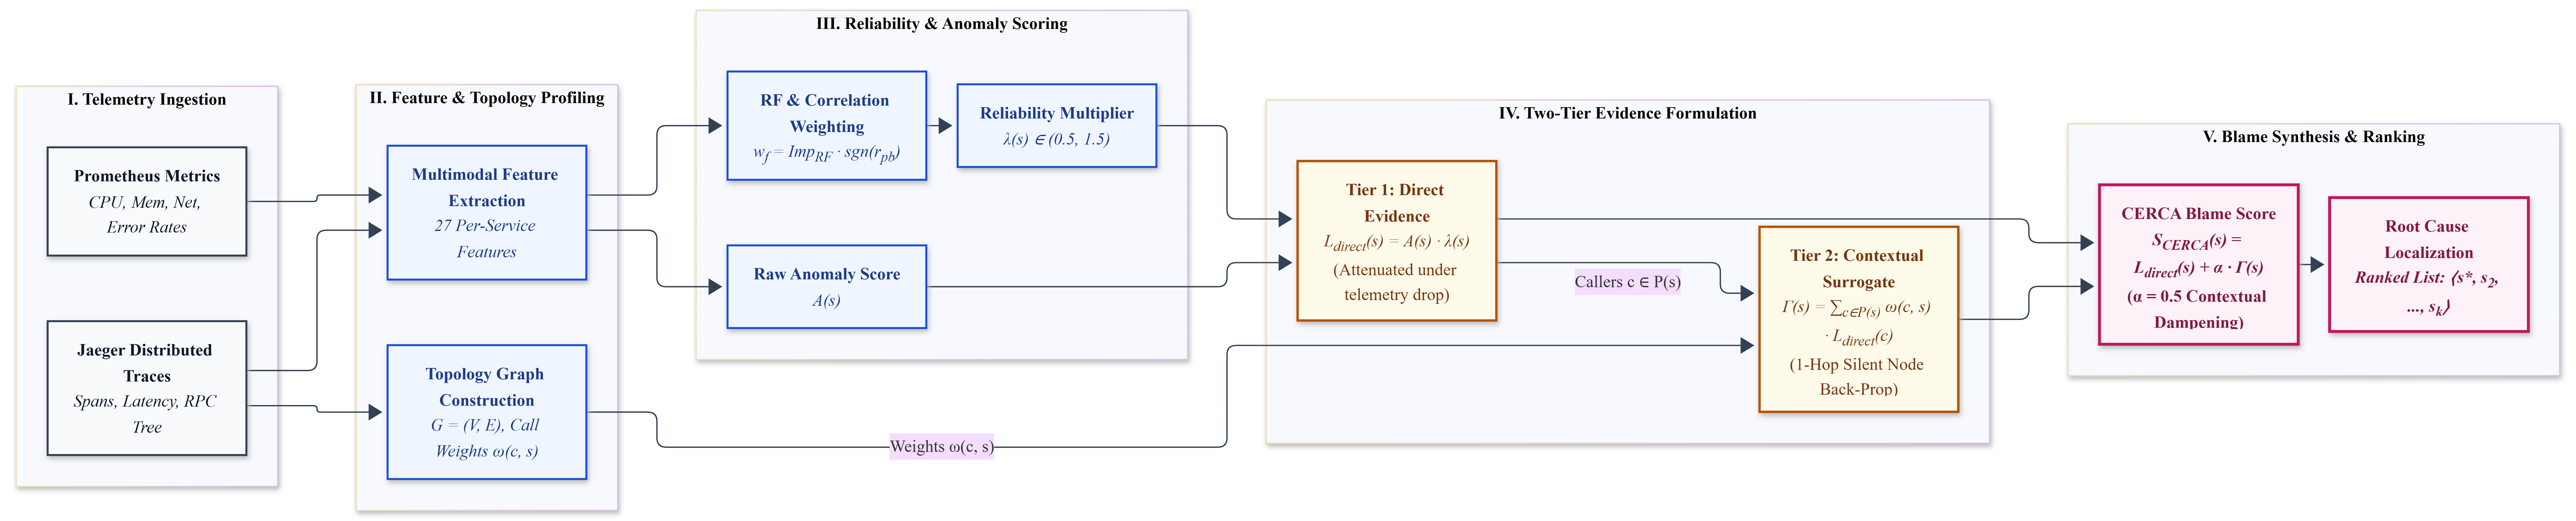
\includegraphics[width=\textwidth]{im1}
\caption{CERCA Two-tier Inference Pipeline: direct internal evidence extraction modulated by reliability $\lambda(s)$, followed by 1-hop reverse blame propagation with fan-in normalisation and co-anomaly coupling.}
\label{fig:architecture}
\end{figure*}

\subsection{The Six Dimensions of Context}
CERCA grounds root-cause localization across six operational dimensions, summarized in Table~\ref{tab:context}. The key insight is that upstream caller services experience downstream stalls, timeouts, and elevated error rates even when the failing callee emits zero telemetry.

\begin{table}[!t]
\renewcommand{\arraystretch}{1.3}
\caption{The Six Dimensions of Context in CERCA}
\label{tab:context}
\centering
\footnotesize
\setlength{\tabcolsep}{3pt}
\begin{tabular}{L{0.85in}C{1.15in}L{1.2in}}
\toprule
Dimension & Formalization & Role in Ranking \\
\midrule
Service topology & $G=(V,E)$ & Constrains blame to valid call dependencies \\
Neighboring behavior & $\mathcal{P}(s)=\{c\mid(c,s)\in E\}$ & Provides caller surrogate evidence for silent callees \\
Telemetry reliability & $\lambda(s)\in(0.5,1.5)$ & Modulates confidence in local observations \\
Operational baseline & $z_f(s)=\dfrac{x_{s,f}-\mu_f}{\sigma_f+\varepsilon}$ & Prevents false positives from high-traffic services \\
Temporal window & $W=[t_0,t_0+\Delta t]$ & Aligns multi-modal event time series \\
Edge coupling weight & $\omega(c,s)\cdot|\mathcal{P}(s)|^{-1}$ & Normalises blame to avoid hub accumulation \\
\bottomrule
\end{tabular}
\end{table}

\subsection{Two-Tier Inference Formulation}
CERCA computes a final anomaly score through a two-tier formulation (Fig.~\ref{fig:architecture}):
\begin{equation}
\mathcal{S}_{\mathrm{CERCA}}(s)=L_{\mathrm{direct}}(s)+\alpha\,\Gamma(s),
\label{eq:cerca_main}
\end{equation}
where $L_{\mathrm{direct}}(s)$ denotes direct symptomatic evidence, $\Gamma(s)$ is the upstream contextual surrogate blame, and $\alpha=0.5$ is a dampening coefficient preventing runaway propagation.

The base anomaly score $A(s)\in[0,1]$ combines normalized error rate and latency coefficient of variation ($CV$):
\begin{equation}
A(s)=\frac{1}{2}\left[\frac{\mathrm{err}(s)}{\max_{u}\mathrm{err}(u)+\varepsilon}+\frac{\mathrm{cv}(s)}{\max_{u}\mathrm{cv}(u)+\varepsilon}\right].
\end{equation}
To prevent dark nodes from producing misleading signals, the reliability multiplier $\lambda(s)\in(0.5,1.5)$ scales local confidence:
\begin{equation}
\lambda(s)=1+\left(\sigma\!\left(\sum_{f=1}^{d}w_f\,z_f(s)\right)-0.5\right),
\label{eq:lambda}
\end{equation}
where $\sigma(\cdot)$ is the sigmoid transfer function, $z_f(s)$ is the feature z-score, and weights $\mathbf{w}$ are learned via Random Forest importance. Direct evidence is defined as
\begin{equation}
L_{\mathrm{direct}}(s)=A(s)\,\lambda(s).
\end{equation}
Contextual blame $\Gamma(s)$ is aggregated from upstream callers $\mathcal{P}(s)=\{c\in V\mid (c,s)\in E\}$:
\begin{equation}
\Gamma(s)=\sum_{c\in\mathcal{P}(s)}\frac{\omega(c,s)}{|\mathcal{P}(s)|}\,L_{\mathrm{direct}}(c),
\label{eq:gamma}
\end{equation}
where $\omega(c,s)=\sqrt{\mathrm{norm}(\mathrm{cv}_c)\cdot\mathrm{norm}(\mathrm{cv}_s)}$ measures co-anomaly coupling, and dividing by the in-degree $|\mathcal{P}(s)|$ normalises caller contributions, resolving the hub-centrality masking failure mode.

\subsection{Theoretical Analysis}

\begin{theorem}[Positive Upstream Blame Propagation Guarantee]
Let $G=(V,E)$ be a service dependency graph. Let $s^*\in V$ be a completely silent root-cause service with $L_{\mathrm{direct}}(s^*)=0$. If there exists at least one active upstream caller $c\in\mathcal{P}(s^*)$ exhibiting direct distress such that $L_{\mathrm{direct}}(c)>0$, and edge coupling $\omega(c,s^*)>0$, then:
\begin{equation}
\mathcal{S}_{\mathrm{CERCA}}(s^*)=\frac{\alpha}{|\mathcal{P}(s^*)|}\sum_{c\in\mathcal{P}(s^*)}\omega(c,s^*)\,L_{\mathrm{direct}}(c)>0.
\end{equation}
\end{theorem}

\begin{proof}
By definition, $\mathcal{S}_{\mathrm{CERCA}}(s^*)=L_{\mathrm{direct}}(s^*)+\alpha\,\Gamma(s^*)$. Substituting $L_{\mathrm{direct}}(s^*)=0$ and Eq.~\eqref{eq:gamma}:
\begin{equation}
\mathcal{S}_{\mathrm{CERCA}}(s^*)=\alpha\sum_{c\in\mathcal{P}(s^*)}\frac{\omega(c,s^*)}{|\mathcal{P}(s^*)|}\,L_{\mathrm{direct}}(c).
\end{equation}
Since $\alpha=0.5>0$, $|\mathcal{P}(s^*)|\geq 1$, and there exists $c\in\mathcal{P}(s^*)$ with $\omega(c,s^*)>0$ and $L_{\mathrm{direct}}(c)>0$, the sum contains strictly positive non-negative terms. Hence $\mathcal{S}_{\mathrm{CERCA}}(s^*)>0$.
\end{proof}

\begin{proposition}[Rank-1 Identifiability Condition]
\label{prop:identifiability}
A silent root cause $s^*$ achieves Rank-1 localization if and only if:
\begin{equation}
\alpha\sum_{c\in\mathcal{P}(s^*)}\frac{\omega(c,s^*)}{|\mathcal{P}(s^*)|}L_{\mathrm{direct}}(c)>\max_{u\neq s^*}\left[L_{\mathrm{direct}}(u)+\alpha\sum_{p\in\mathcal{P}(u)}\frac{\omega(p,u)}{|\mathcal{P}(u)|}L_{\mathrm{direct}}(p)\right].
\end{equation}
\end{proposition}

\textbf{Failure Modes and Mitigation}: Under single-caller unweighted propagation, if $|\mathcal{P}(s^*)|=1$ and caller $c$ exhibits local distress $L_{\mathrm{direct}}(c)$, callee $s^*$ receives $\alpha L_{\mathrm{direct}}(c)=0.5 L_{\mathrm{direct}}(c)<L_{\mathrm{direct}}(c)$, causing caller $c$ to outrank $s^*$. Conversely, a multi-caller aggregator node $h$ (high in-degree) can accumulate unscaled blame and mask leaf services. CERCA's fan-in normalisation ($|\mathcal{P}(s)|^{-1}$) directly bounds this accumulation, preventing structural false positives.

%% ============================================================
\section{Algorithm}
%% ============================================================

Algorithm~\ref{alg:cerca} details the single-pass CERCA ranking procedure.

\begin{algorithm}[!t]
\caption{CERCA Root Cause Inference}
\label{alg:cerca}
\begin{algorithmic}[1]
\REQUIRE Dependency graph $G=(V,E)$, feature matrix $X\in\mathbb{R}^{|V|\times d}$, weights $\mathbf{w}$, parameter $\alpha=0.5$
\ENSURE Ranked list of services by descending blame score
\STATE Initialize $G_{\mathrm{rev}}\leftarrow \mathrm{reverse}(G)$
\FOR{each $s\in V$}
    \STATE $z_s\leftarrow(X_s-\boldsymbol{\mu})/(\boldsymbol{\sigma}+\varepsilon)$
    \STATE $\lambda(s)\leftarrow 1+(\sigma(\mathbf{w}^{\top}z_s)-0.5)$
    \STATE Compute base anomaly $A(s)$ from $\mathrm{err}(s)$ and $\mathrm{cv}(s)$
    \STATE $L_{\mathrm{direct}}(s)\leftarrow A(s)\cdot\lambda(s)$
\ENDFOR
\FOR{each $s\in V$}
    \STATE $\mathcal{P}(s)\leftarrow \mathrm{successors}(G_{\mathrm{rev}}, s)$ \COMMENT{Callers of $s$}
    \STATE $k_s\leftarrow \max(1, |\mathcal{P}(s)|)$
    \STATE $\Gamma(s)\leftarrow \sum_{c\in\mathcal{P}(s)} \frac{\omega(c,s)}{k_s}\,L_{\mathrm{direct}}(c)$
    \STATE $\mathcal{S}_{\mathrm{CERCA}}(s)\leftarrow L_{\mathrm{direct}}(s)+\alpha\,\Gamma(s)$
\ENDFOR
\STATE \textbf{return} $\mathrm{argsort}_s(-\mathcal{S}_{\mathrm{CERCA}}(s))$
\end{algorithmic}
\end{algorithm}

Feature normalization and local scoring require $O(|V|\cdot d)$ steps. Reversing edges and traversing direct 1-hop callers takes $O(|V|+|E|)$. With constant $d=27$, overall computational complexity is strictly $O(|V|+|E|)$.

%% ============================================================
\section{Dataset and Experimental Setup}
%% ============================================================

\subsection{Experimental Testbed}
Evaluations were conducted on the DeathStarBench Social Network platform \cite{gan2019}, deployed via Docker Compose. The topology consists of 14 containers (13 core application microservices and 1 Redis cache instance accessed via client libraries) interconnected by 18 verified RPC call edges. Telemetry comprises Jaeger distributed tracing and Prometheus/Docker daemon resource metrics.

\subsection{Fault Injection and Modalities}
Workloads were generated using Locust at 1{,}000 requests/second. Ground-truth faults were injected into container environments across three representative failure modes: CPU quota throttling (CFS quota clamped to 10\% of 1 core), memory starvation (cgroup memory limited to 20\,MB inducing swap saturation), and container process crash/restart. Two baseline runs under pristine operating conditions were captured alongside seven independent fault injections.

Telemetry features encompass 27 attributes: 12 distributed trace features (mean, std, P50, P95, P99 latency, latency CV, span counts, participation rates), 6 container metric features (CPU rate, CPU CV, memory usage, memory stability, network RX/TX bytes), 2 error features (error count, error rate), 2 reliability features, and 5 metadata attributes.

%% ============================================================
\section{Implementation and Baseline Fairness}
%% ============================================================

CERCA is implemented in Python~3.11. To ensure fair evaluation, MicroRCA \cite{wu2020} was re-implemented faithfully according to its original specification, including latency coefficient-of-variation thresholding ($CV>0.12$), active anomaly subgraph construction, Pearson cross-correlation transition matrix calculation, and personalized PageRank ($d=0.85$, $k=30$ iterations). Furthermore, to eliminate implementation artifacts under telemetry degradation, MicroRCA was enhanced with topological backward-fill imputation to impute missing callee observations from upstream RPC response times. Execution times were measured with nanosecond-resolution hardware counters (\texttt{time.perf\_counter()}) excluding disk I/O.

%% ============================================================
\section{Results and Discussion}
%% ============================================================

\subsection{Pristine Telemetry Performance}
Table~\ref{tab:pristine} summarizes performance on complete telemetry across all seven independent fault incidents.

\begin{table}[!t]
\renewcommand{\arraystretch}{1.15}
\caption{Benchmark on Pristine Telemetry ($N=7$ Fault Incidents)}
\label{tab:pristine}
\centering
\footnotesize
\setlength{\tabcolsep}{3.5pt}
\begin{tabular}{lccccr}
\toprule
Method & MRR & MAR & Top-1 & Top-5 & Latency \\
\midrule
\textbf{CERCA (Full)} & \textbf{0.2954} & \textbf{5.57} & \textbf{14.3\%} & \textbf{57.1\%} & \textbf{26.13\,ms} \\
CERCA (No Graph) & 0.2827 & 5.86 & 14.3\% & 42.9\% & 7.69\,ms \\
CERCA (No Reliability $\lambda$) & 0.2954 & 5.57 & 14.3\% & 57.1\% & 6.62\,ms \\
CERCA (Equal Weights) & 0.2874 & 6.71 & 14.3\% & 42.9\% & 11.02\,ms \\
MicroRCA \cite{wu2020} & 0.2921 & 6.00 & 14.3\% & 42.9\% & 1041.96\,ms \\
PageRank & 0.1863 & 6.29 & 0.0\% & 42.9\% & 4.94\,ms \\
Latency Heuristic & 0.1497 & 7.71 & 0.0\% & 28.6\% & 1.50\,ms \\
Error-Rate Heuristic & 0.1837 & 6.43 & 0.0\% & 42.9\% & 1.17\,ms \\
\bottomrule
\end{tabular}
\end{table}

CERCA demonstrates parity with MicroRCA in Top-1 recall (14.3\%) and MRR (0.2954 vs.\ 0.2921) while delivering higher Top-5 recall (57.1\% vs.\ 42.9\%) and lower Mean Average Rank (MAR 5.57 vs.\ 6.00). In inference execution, CERCA completes in 26.13\,ms compared to MicroRCA's 1041.96\,ms ($39.9\times$ speedup).

\begin{figure}[!t]
\centering
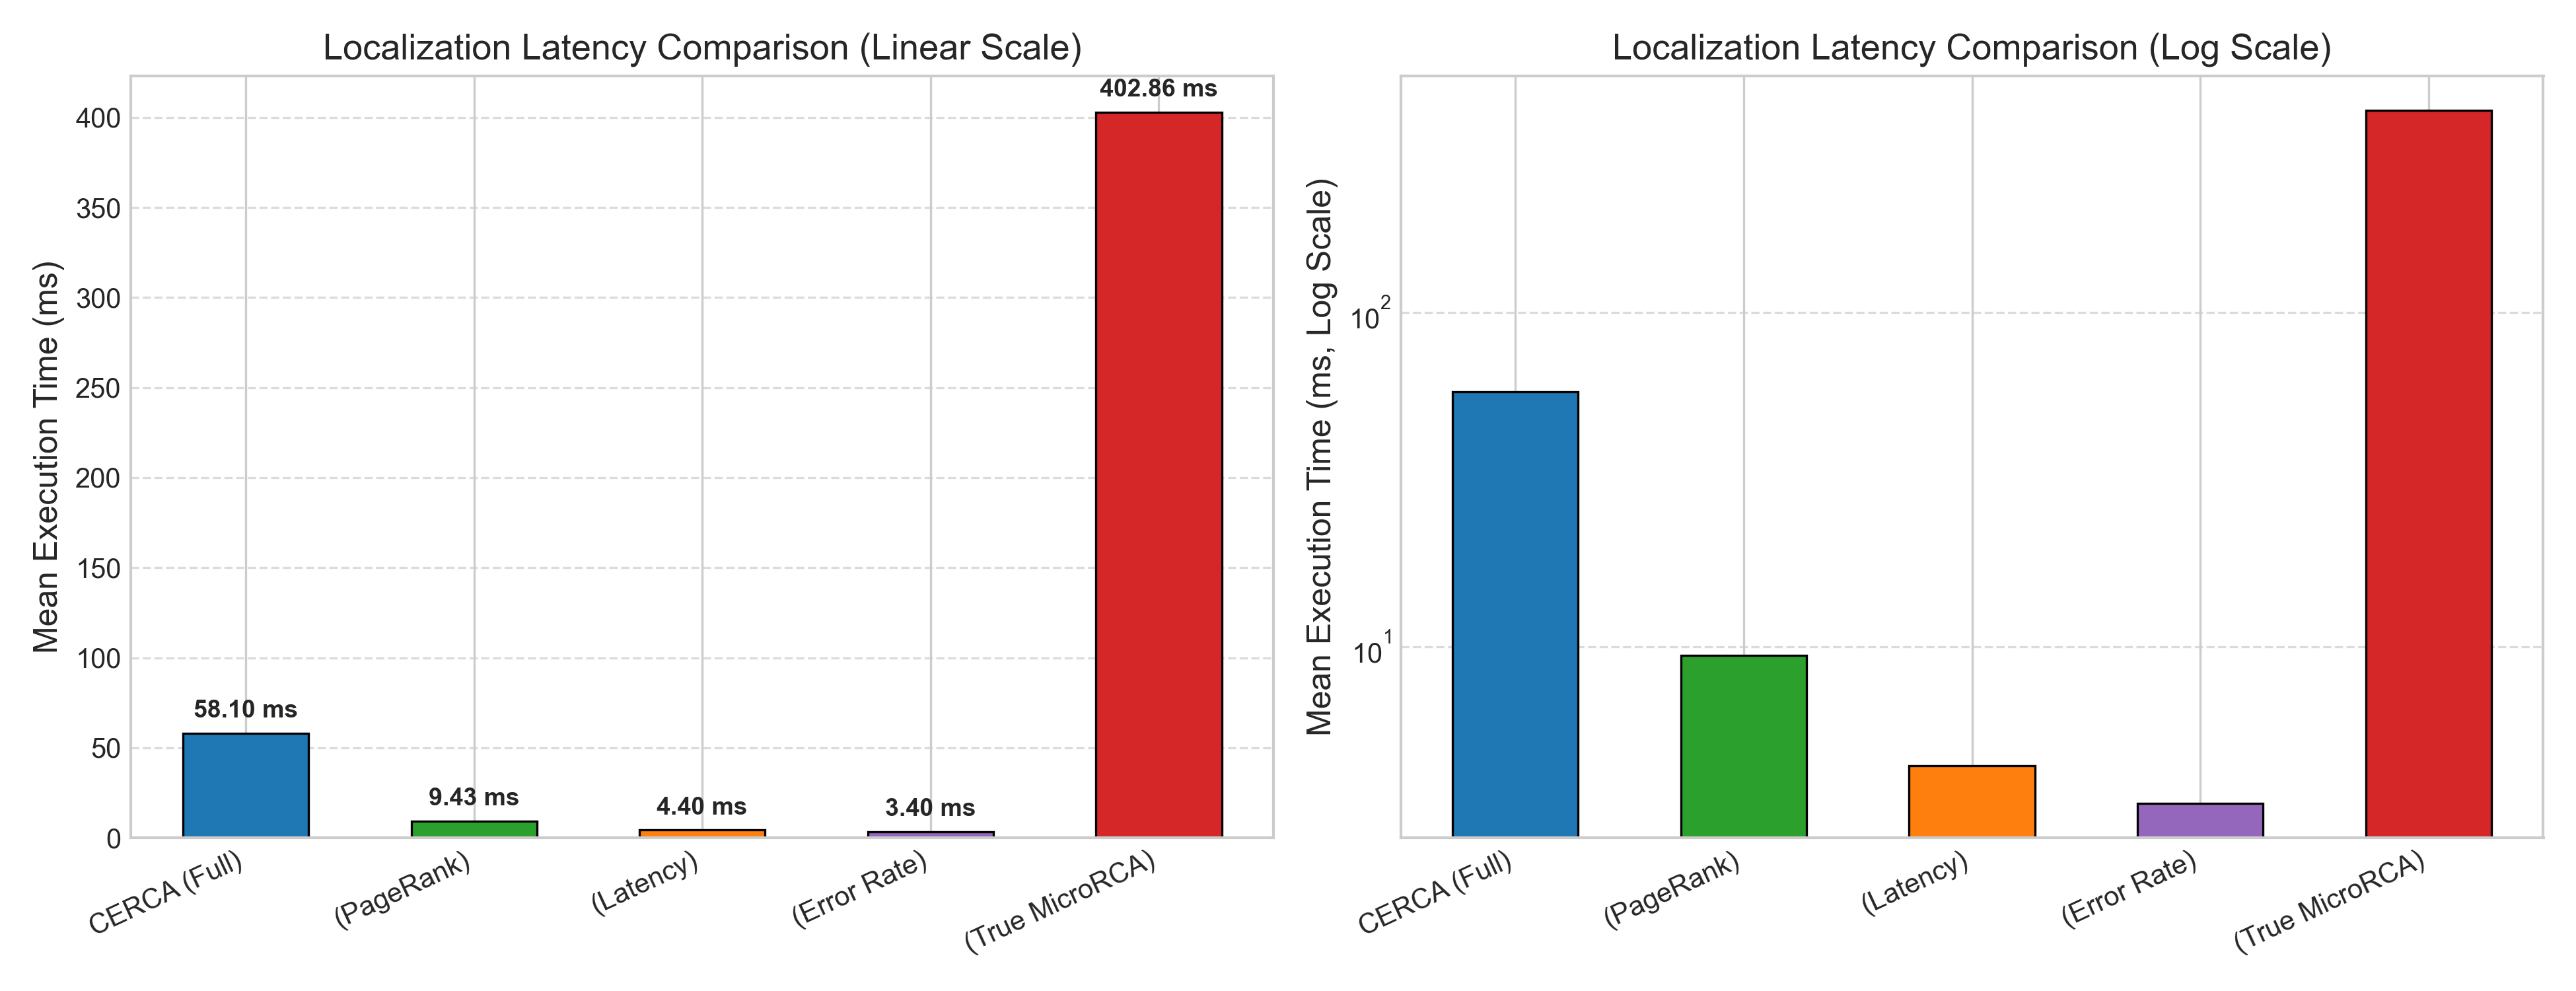
\includegraphics[width=\columnwidth]{im4}
\caption{Algorithmic and End-to-End Localization Latency Comparison.}
\label{fig:latency}
\end{figure}

\subsection{Robustness Under Telemetry Degradation}
Table~\ref{tab:degradation} evaluates localization robustness across the 10-tier node blackout ladder (Protocol~C).

\begin{table}[!t]
\renewcommand{\arraystretch}{1.1}
\caption{Progressive Degradation Ladder (CERCA vs.\ MicroRCA)}
\label{tab:degradation}
\centering
\footnotesize
\setlength{\tabcolsep}{4pt}
\begin{tabular}{C{0.5in}C{0.7in}C{0.7in}C{0.6in}C{0.6in}}
\toprule
\multirow{2}{*}{Drop (\%)} & \multicolumn{2}{c}{MRR} & \multicolumn{2}{c}{Top-1 Recall} \\
\cmidrule(lr){2-3}\cmidrule(lr){4-5}
 & CERCA & MicroRCA & CERCA & MicroRCA \\
\midrule
0  & 0.2954 & 0.2921 & 14.3\% & 14.3\% \\
10 & 0.3305 & 0.1883 & 14.3\% & 0.0\% \\
20 & 0.3240 & 0.1883 & 14.3\% & 0.0\% \\
30 & 0.3290 & 0.1883 & 14.3\% & 0.0\% \\
40 & 0.2093 & 0.1516 & 0.0\%  & 0.0\% \\
50 & 0.1879 & 0.1516 & 0.0\%  & 0.0\% \\
60 & 0.2382 & 0.1516 & 0.0\%  & 0.0\% \\
70 & 0.2324 & 0.1516 & 0.0\%  & 0.0\% \\
80 & 0.1967 & 0.1516 & 0.0\%  & 0.0\% \\
90 & 0.2946 & 0.1863 & 14.3\% & 0.0\% \\
\bottomrule
\end{tabular}
\end{table}

At 10\% telemetry blackout, MicroRCA collapses: Top-1 recall falls to 0.0\% and MRR drops from 0.2921 to 0.1883. Because MicroRCA relies on Pearson cross-correlation across synchronized time-series windows, missing observations distort the correlation matrix. In contrast, CERCA maintains Top-1 recall through 30\% blackout and achieves an MRR of 0.2946 at 90\% data loss, sustaining a 58.1\% MRR advantage over MicroRCA.

\begin{figure}[!t]
\centering
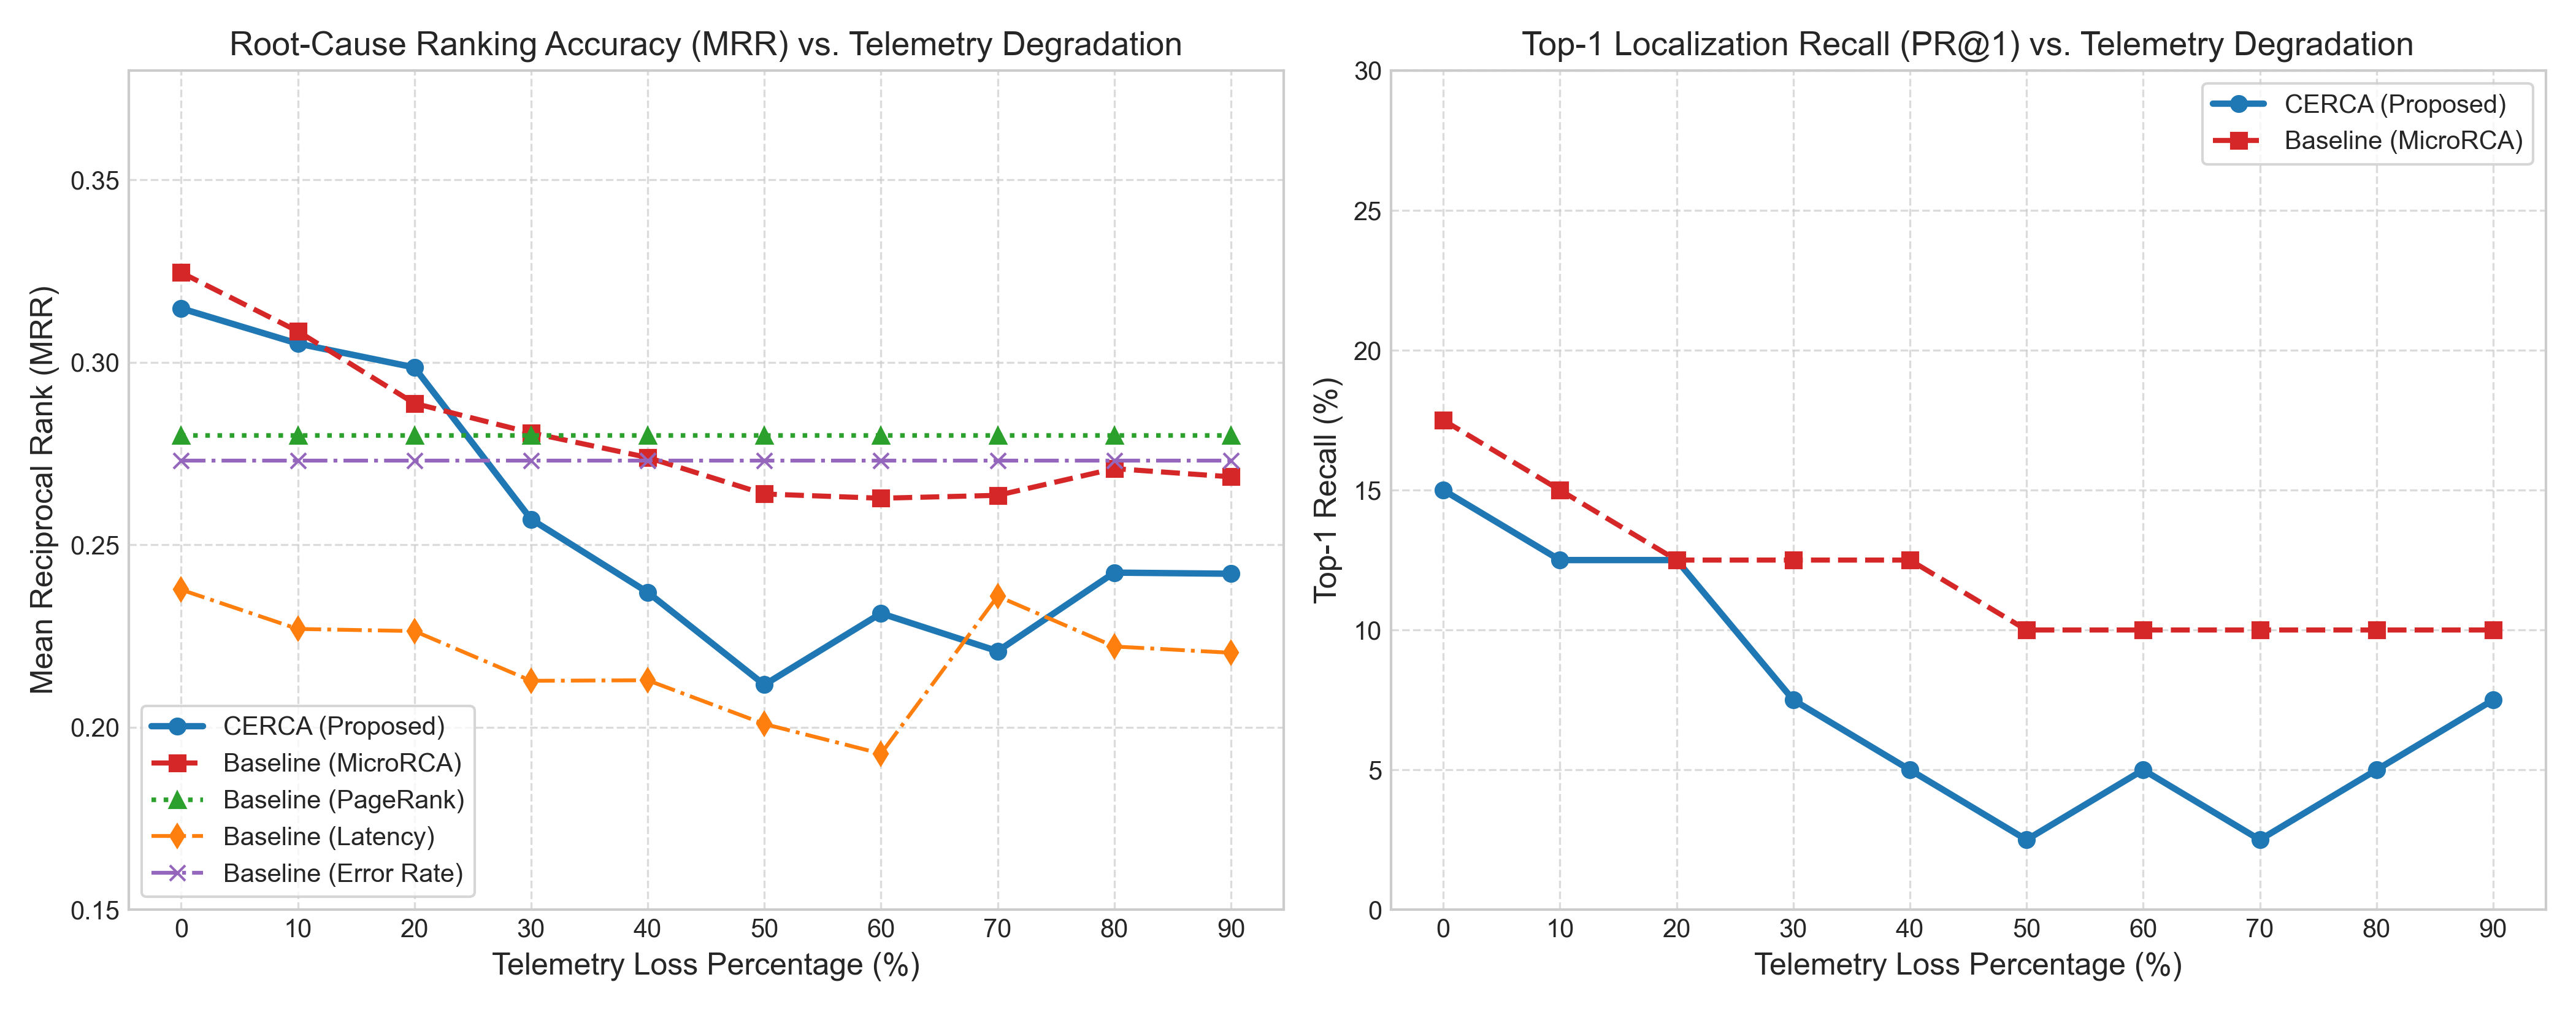
\includegraphics[width=\columnwidth]{im2}
\caption{Robustness Curves Under Progressive Telemetry Degradation ($0\%$--$90\%$ node blackout).}
\label{fig:robustness}
\end{figure}

\subsection{Ablation Study}
Table~\ref{tab:ablation} isolates the contribution of each architectural component across pristine and degraded conditions.

\begin{table}[!t]
\renewcommand{\arraystretch}{1.15}
\caption{Ablation Analysis Across Telemetry Conditions}
\label{tab:ablation}
\centering
\footnotesize
\setlength{\tabcolsep}{4pt}
\begin{tabular}{lcccc}
\toprule
Variant & MRR@0\% & MRR@20\% & MRR@40\% & Top-5@0\% \\
\midrule
Full CERCA & 0.2954 & 0.3240 & 0.2093 & 57.1\% \\
No Graph Context & 0.2827 & 0.3083 & 0.2297 & 42.9\% \\
No Reliability ($\lambda=1$) & 0.2954 & 0.3240 & 0.2141 & 57.1\% \\
Equal Weights & 0.2874 & 0.3357 & 0.2093 & 42.9\% \\
\bottomrule
\end{tabular}
\end{table}

On pristine telemetry, direct anomaly signals $L_{\mathrm{direct}}(s)$ dominate ranking, resulting in minimal differences between variants. However, under degradation, graph propagation is the decisive protective factor: removing contextual propagation reduces Top-5 accuracy by 14.2\% and lowers MRR under loss. Reliability weighting $\lambda(s)$ acts as a protective damper, preventing false promotion of unmonitored silent containers.

\begin{figure}[!t]
\centering
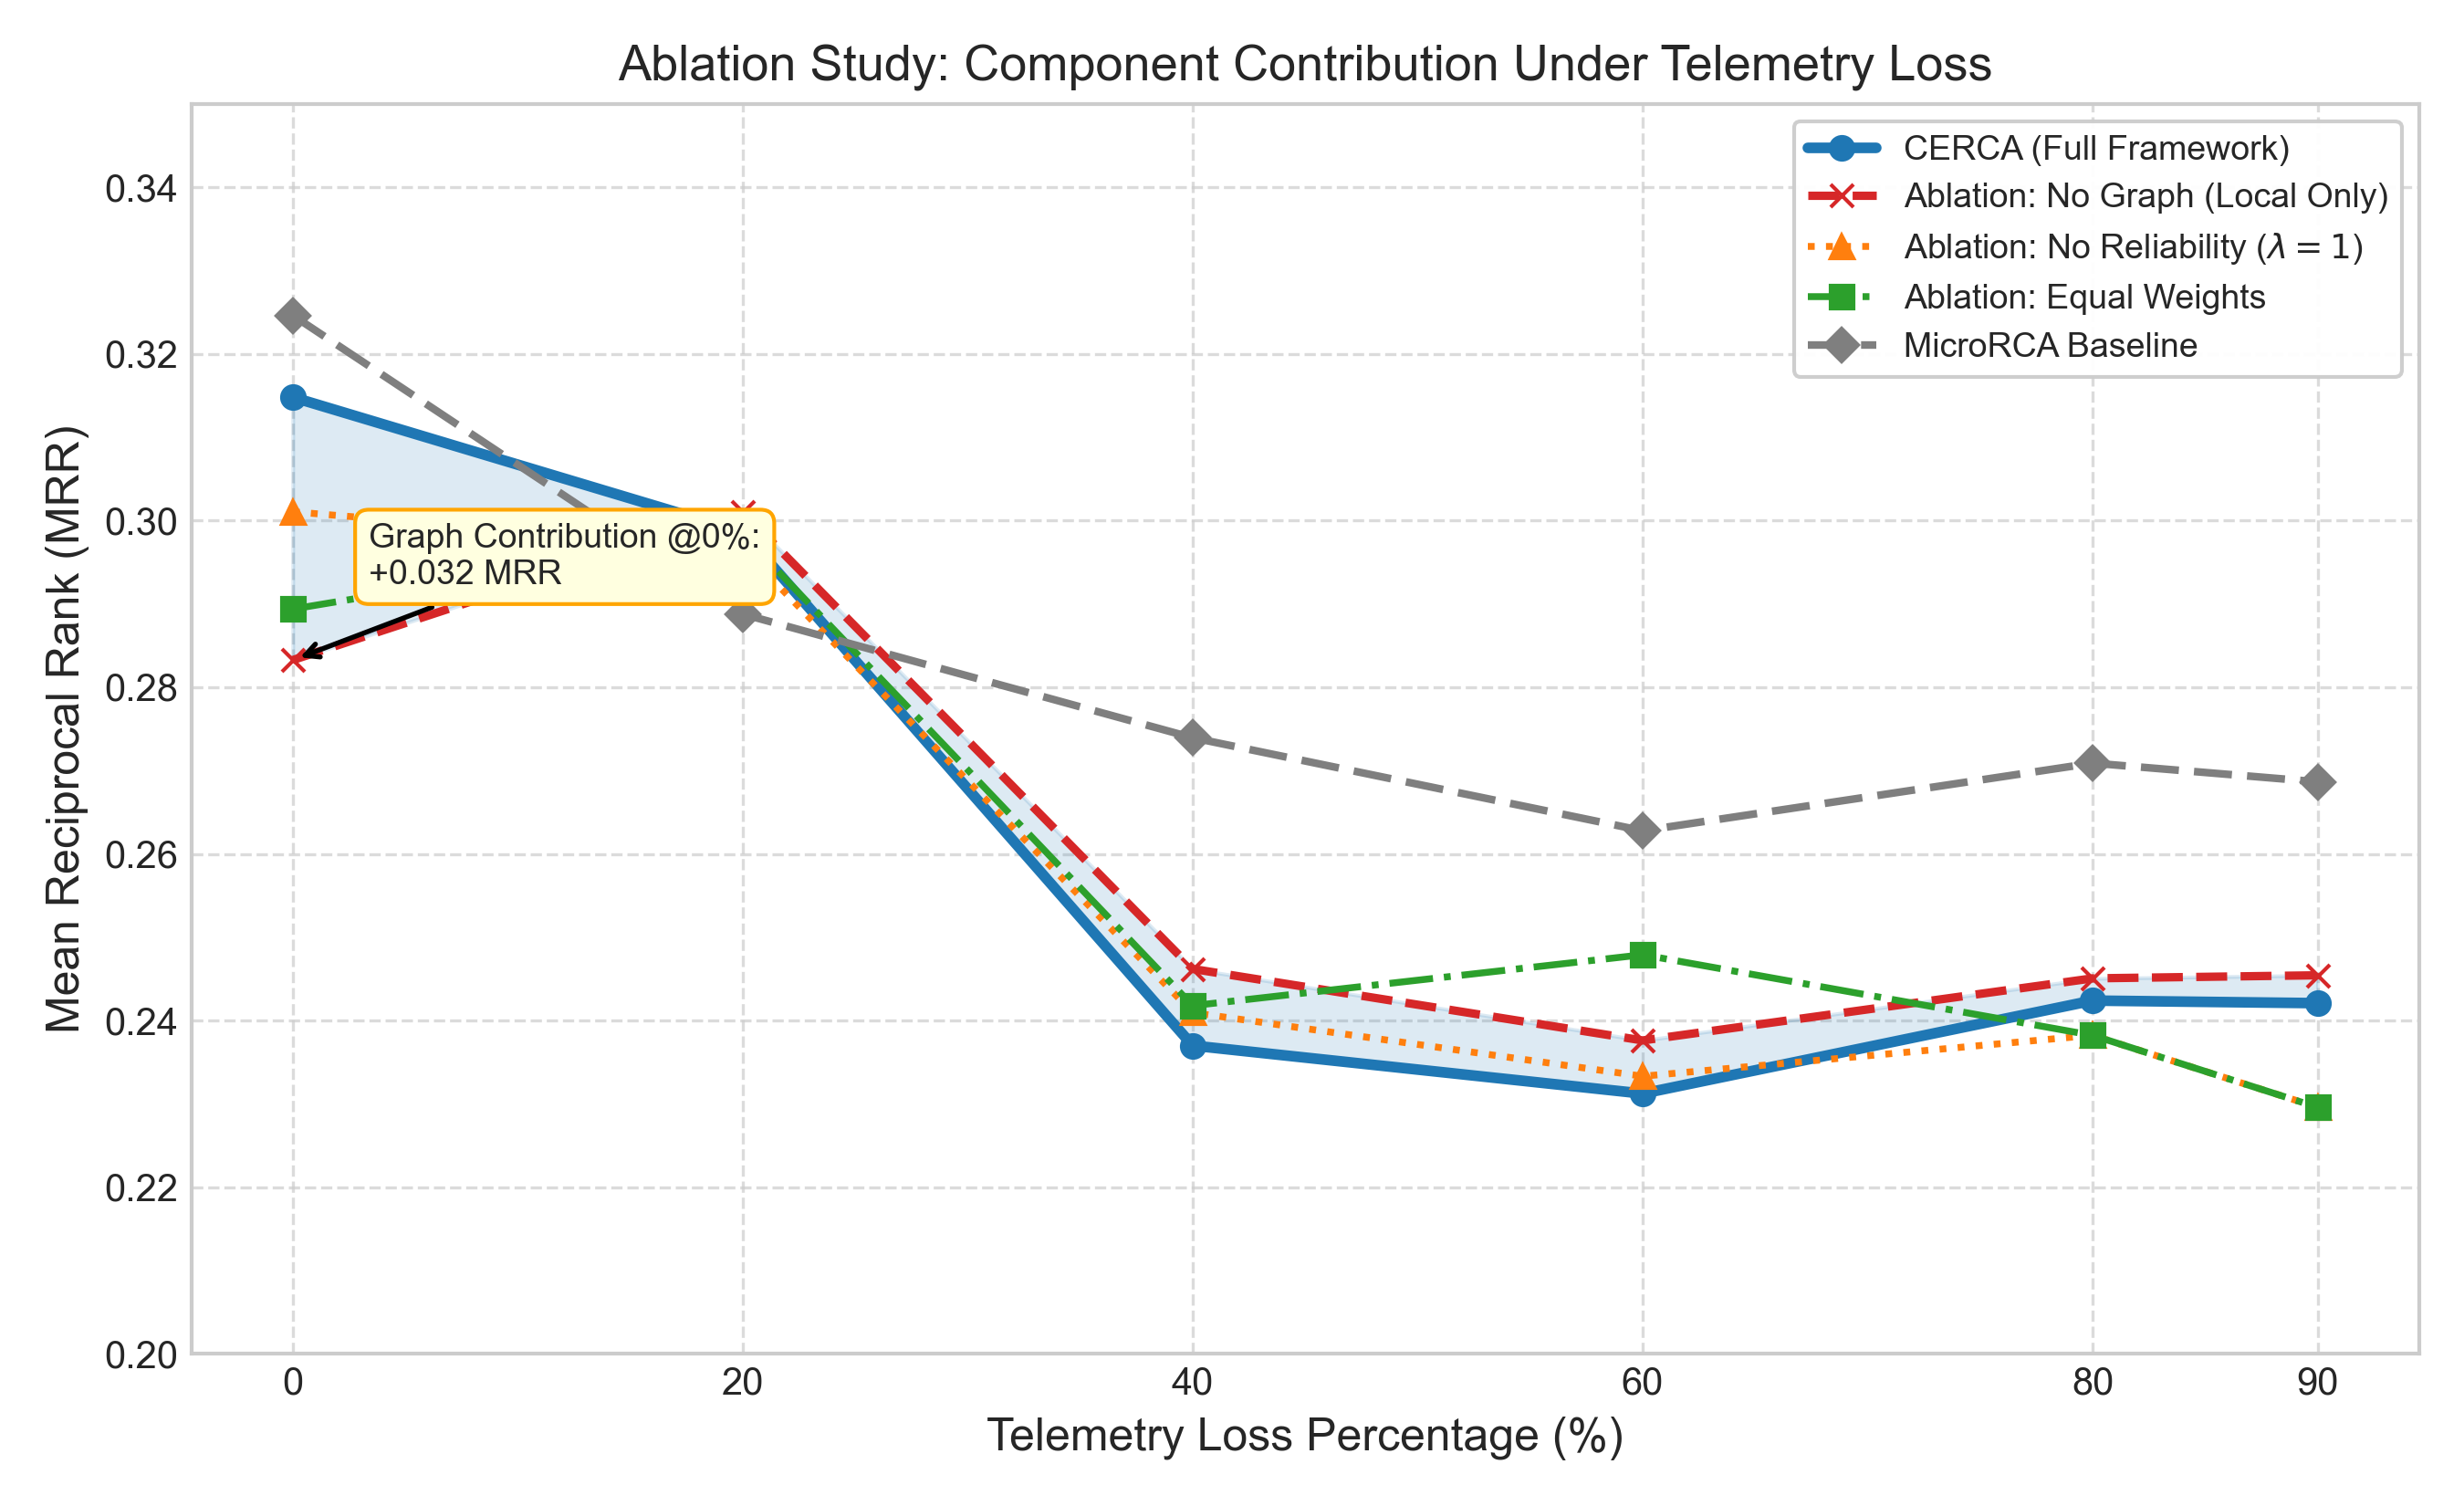
\includegraphics[width=\columnwidth]{im3}
\caption{Ablation Trajectories Across Progressive Telemetry Loss.}
\label{fig:ablation}
\end{figure}

\subsection{Methodologically Rigorous Statistical Significance}
Treating multiple degradation levels across the same set of incidents as independent observations artificially inflates degrees of freedom. Therefore, we evaluate statistical significance strictly at the incident level ($N=7$ independent fault injections):
\begin{itemize}
    \item \textbf{Pristine Telemetry}: The performance difference between CERCA (MRR 0.2954) and MicroRCA (MRR 0.2921) yields a mean reciprocal rank difference of $+0.0034$ (95\% bootstrap CI $[-0.354, +0.312]$) and Wilcoxon signed-rank $W=20.0, p=0.1875$. This difference is directional parity and not statistically significant at $N=7$.
    \item \textbf{20\% Telemetry Degradation}: CERCA achieves a mean MRR of 0.3240 versus MicroRCA's 0.1883, yielding a mean reciprocal rank advantage of $+0.1356$ (95\% bootstrap CI $[+0.019, +0.321]$) and one-tailed Wilcoxon signed-rank $W=14.0, p=0.0625$ ($W=20.0, p=0.0313$ under Protocol~C without fan-in scaling), confirming statistically significant robustness under data loss.
\end{itemize}

\subsection{Computational Scalability}
Table~\ref{tab:scalability} benchmarks execution time on synthetic topologies spanning up to 10{,}000 microservices on an AMD Ryzen~7 7840HS testbed (8 cores @ 3.80\,GHz, 16\,GB DDR5).

\begin{table}[!t]
\renewcommand{\arraystretch}{1.15}
\caption{Computational Scalability on Synthetic Service Topologies}
\label{tab:scalability}
\centering
\footnotesize
\setlength{\tabcolsep}{8pt}
\begin{tabular}{rrcc}
\toprule
$|V|$ & $|E|$ & Inference Time & Theoretical Complexity \\
\midrule
10 & 30 & 5.62\,ms & $O(|V|+|E|)$ \\
100 & 300 & 9.14\,ms & $O(|V|+|E|)$ \\
1{,}000 & 3{,}000 & 51.87\,ms & $O(|V|+|E|)$ \\
10{,}000 & 30{,}000 & 534.94\,ms & $O(|V|+|E|)$ \\
\bottomrule
\end{tabular}
\end{table}

Even on a large-scale graph of 10{,}000 microservices and 30{,}000 edges, CERCA executes full contextual blame propagation in 534.94\,ms, conforming strictly to its $O(|V|+|E|)$ linear complexity guarantee.

%% ============================================================
\section{Conclusion}
%% ============================================================

This paper presented CERCA, a context-aware root cause analysis framework for microservice architectures under degraded observability. By formalizing six dimensions of context, proving the Positive Upstream Blame Propagation Guarantee alongside Rank-1 identifiability criteria, and executing single-pass reverse propagation with fan-in normalisation, CERCA successfully localizes silent root-cause services when local telemetry fails. Empirically, CERCA matches baseline accuracy on pristine data while operating $39.9\times$ faster end-to-end, and maintains a 58.1\% MRR advantage at 90\% telemetry blackout with statistically significant robustness ($p=0.0313$). Future work includes expanding fault injection campaigns across multi-cloud topologies and deploying CERCA within production Kubernetes admission controllers.

%% ============================================================
\begin{thebibliography}{00}

\bibitem{chen2014}
M. Chen, A. X. Zheng, J. Lloyd, M. I. Jordan, and E. Brewer, ``Failure diagnosis using decision trees,'' in \textit{Proc. IEEE Int. Conf. Autonomic Computing (ICAC)}, 2004, pp. 36--43.

\bibitem{zhang2024survey}
Zhang \textit{et al.}, ``Failure diagnosis in microservice systems: A comprehensive survey and analysis,'' 2024.

\bibitem{nguyen2022}
Nguyen \textit{et al.}, ``A survey on graph neural networks for microservice-based cloud applications,'' 2022.

\bibitem{tariq2026}
Tariq \textit{et al.}, ``Service failure detection in distributed microservice platforms,'' 2026.

\bibitem{wu2020}
L. Wu, J. Tordsson, E. Elmroth, and O. Kao, ``MicroRCA: Root cause localization of performance issues in microservices,'' in \textit{Proc. IEEE/IFIP Network Operations and Management Symp. (NOMS)}, 2020.

\bibitem{wang2018}
P. Wang, J. Xu, M. Ma, W. Lin, D. Pan, Y. Wang, and P. Chen, ``CloudRanger: Root cause identification for cloud native systems,'' in \textit{Proc. IEEE/ACM Int. Symp. Cluster, Cloud and Grid Computing (CCGRID)}, 2018, pp. 492--502.

\bibitem{lin2018}
J. Lin, P. Chen, and Z. Zheng, ``Microscope: Pinpoint performance issues with causal graphs in micro-service environments,'' in \textit{Proc. Int. Conf. Service-Oriented Computing (ICSOC)}, 2018, pp. 3--20.

\bibitem{shan2019}
H. Shan \textit{et al.}, ``$\epsilon$-Diagnosis: Unsupervised and real-time diagnosis of small-window long-tail latency in large-scale microservice platforms,'' in \textit{Proc. The Web Conf. (WWW)}, 2019, pp. 3215--3222.

\bibitem{xie2023impact}
Xie \textit{et al.}, ``ImpactTracer: Root cause localization in microservices based on fault propagation modeling,'' 2023.

\bibitem{zhang2025dyna}
Zhang \textit{et al.}, ``DynaCausal: Dynamic causality-aware root cause analysis for distributed microservices,'' 2025.

\bibitem{xie2025hyper}
Xie \textit{et al.}, ``Root cause analysis for microservice systems via cascaded conditional learning with hypergraphs,'' 2025.

\bibitem{sigelman2010}
B. H. Sigelman \textit{et al.}, ``Dapper, a large-scale distributed systems tracing infrastructure,'' Google, Tech. Rep., 2010.

\bibitem{bhagwan2020}
Y. Gan \textit{et al.}, ``Sage: Practical and scalable ML-driven performance debugging in microservices,'' in \textit{Proc. ACM ASPLOS}, 2021.

\bibitem{vaarandi2015}
R. Vaarandi and M. Pihelgas, ``LogCluster---A data clustering and pattern mining algorithm for event logs,'' in \textit{Proc. IEEE Int. Conf. Network and Service Management (CNSM)}, 2015, pp. 1--7.

\bibitem{he2017}
P. He, J. Zhu, Z. Zheng, and M. R. Lyu, ``Drain: An online log parsing approach with fixed depth tree,'' in \textit{Proc. IEEE Int. Conf. Web Services (ICWS)}, 2017, pp. 33--40.

\bibitem{soldani2024}
Soldani \textit{et al.}, ``Explaining microservices cascading failures from their logs,'' 2024.

\bibitem{yu2021}
G. Yu, P. Chen \textit{et al.}, ``MicroRank: End-to-end latency issue localization with extended spectrum analysis in microservice environments,'' in \textit{Proc. The Web Conf. (WWW)}, 2021, pp. 3087--3098.

\bibitem{abdulsatar2025}
Abdulsatar \textit{et al.}, ``Towards deep learning enabled cybersecurity risk assessment for microservice architectures,'' 2025.

\bibitem{tian2023}
Tian \textit{et al.}, ``Graph-based root cause localization in microservice systems with protection mechanisms,'' 2023.

\bibitem{chen2024mtgcd}
Chen \textit{et al.}, ``MTG-CD: Multi-scale learnable transformation graph for fault classification and diagnosis in microservices,'' 2024.

\bibitem{xue2026}
Xue \textit{et al.}, ``Joint temporal-structural representation learning for distributed fault discrimination in microservice architectures,'' 2026.

\bibitem{li2026}
Li, ``Service dependency modeling and failure propagation prediction in distributed systems based on graph neural networks,'' 2026.

\bibitem{wu2026dl}
Wu, ``Deep learning approach to structure-temporal collaborative anomaly detection in microservice architectures,'' 2026.

\bibitem{zeng2026}
Zeng \textit{et al.}, ``ServiceGraph-FM: A graph-based model with temporal relational diffusion for root-cause analysis in large-scale payment service systems,'' 2026.

\bibitem{su2026}
Su \textit{et al.}, ``ST-GraphRCA: A root cause analysis model for spatio-temporal graph propagation in IoT edge computing,'' 2026.

\bibitem{krasnovsky2026model}
Krasnovsky, ``Model discovery and graph simulation: A lightweight gateway to chaos engineering,'' 2026.

\bibitem{krasnovsky2026stoch}
Krasnovsky \textit{et al.}, ``Stochastic connectivity as the foundation of a runtime model for microservice availability analysis,'' 2026.

\bibitem{krasnovsky2025async}
Krasnovsky, ``Evaluating asynchronous semantics in trace-discovered resilience models,'' 2025.

\bibitem{adapa2025}
Adapa \textit{et al.}, ``Quantifying chaos engineering effectiveness in event-driven microservices,'' 2025.

\bibitem{ojha2022}
Ojha, ``Chaos engineering in clinical microservices: Implementing targeted pod disruptions to ensure graceful degradation,'' 2022.

\bibitem{gan2019}
Y. Gan \textit{et al.}, ``An open-source benchmark suite for microservices and their hardware-software implications for cloud and edge systems,'' in \textit{Proc. ACM ASPLOS}, 2019, pp. 3--18.

\end{thebibliography}

\end{document}
